\documentclass[10pt]{article}
\usepackage[T1]{fontenc}
\usepackage[margin=0.72in]{geometry}
\usepackage{amsmath,amssymb,amsthm}
\usepackage{graphicx}
\usepackage[colorlinks=true,linkcolor=blue,citecolor=blue,urlcolor=blue]{hyperref}
\usepackage{microtype}

\newtheorem{theorem}{Theorem}
\newtheorem{lemma}{Lemma}
\newcommand{\F}{\mathbb F}
\newcommand{\E}{\mathbb E}
\newcommand{\TC}{\operatorname{TC}}

\title{A dimension-free lower bound for total coherence\
of Parseval frames}
\author{Full answer to an open question in arXiv:1910.01733}
\date{13 August 2026}

\begin{document}
\maketitle

\noindent\textbf{Status.}
The source question has an affirmative answer over both \(\mathbb R\) and
\(\mathbb C\).  A Haar-random Parseval frame already has the requested order
of total coherence in expectation.  In particular, one may take the universal
constant
\[
             c=\frac{2\sqrt2}{\pi^{3/2}}=0.5079\ldots.
\]

\section*{Source question}

For an \(M\)-vector Parseval frame
\(\Phi=(\varphi_1,\ldots,\varphi_M)\) in \(\F^N\), the source defines
\[
 \TC(\Phi)=\sum_{i\ne j}|\langle\varphi_i,\varphi_j\rangle|.
\]
It asks whether some \(c>0\), independent of \(N,M\), always permits a
Parseval frame satisfying
\[
 \TC(\Phi)\ge c\sqrt{N(M-N)(M-1)}
 \tag{Q}
\]
\cite[p.~25]{CC}.  The next paragraph explicitly proposes calculating the
expectation for a random Parseval frame.

\begin{center}
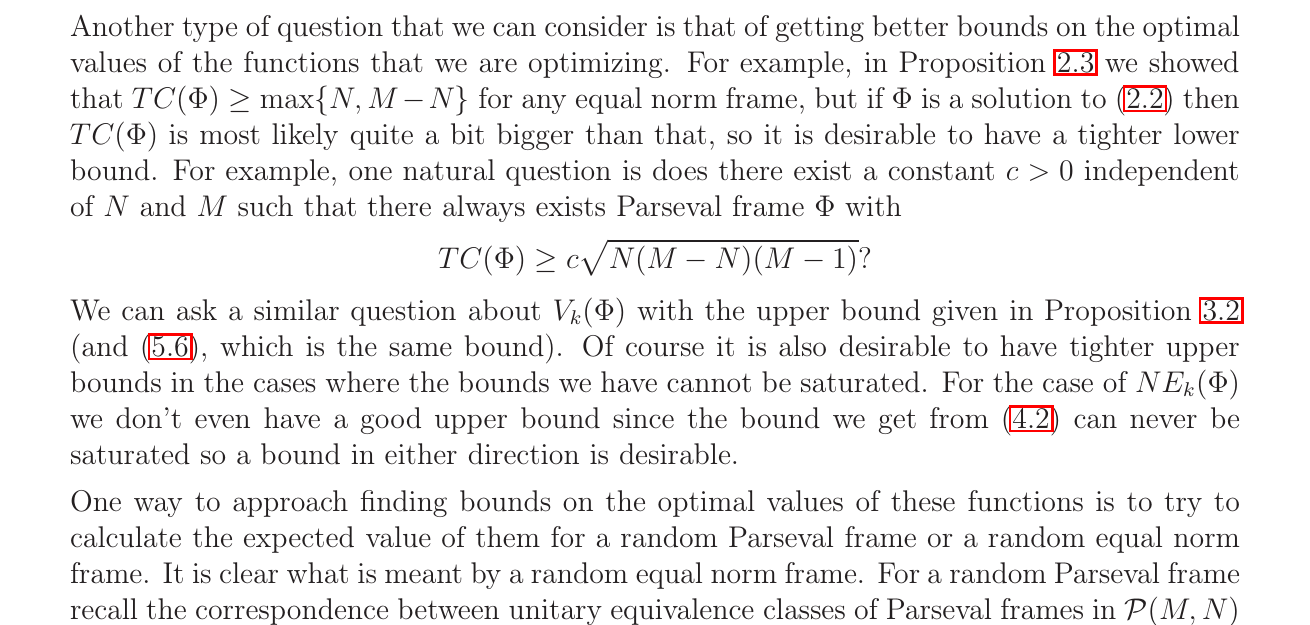
\includegraphics[width=0.96\textwidth]{source/source_question_page25.png}
\end{center}
\vspace{-0.7em}
\noindent\emph{Source evidence: arXiv:1910.01733, PDF page 25.}

\section*{Answer and exact expectations}

Assume \(1\le N<M\), and put
\[
             q=M-N,\qquad D=M-1.
\]
Choose a Haar-uniform \(N\)-dimensional subspace of \(\F^M\), and let \(P\)
be the orthogonal projection onto it.  Choose any Parseval frame \(\Phi\)
whose Gram matrix is \(P\).  (Equivalently, take an \(N\times M\) matrix with
orthonormal rows and Gram matrix \(P\).)

\begin{theorem}\label{thm:main}
For the random Parseval frame above, if \(\F=\mathbb C\), then
\begin{equation}\label{eq:complex-exact}
 \E\TC(\Phi)=
 D\frac{\Gamma(N+\tfrac12)}{\Gamma(N)}
   \frac{\Gamma(q+\tfrac12)}{\Gamma(q)}
   \frac{\Gamma(\tfrac32)\Gamma(D)}{\Gamma(D+\tfrac12)}
 \ge \frac{\pi^{3/2}}8\sqrt{NqD}.
\end{equation}
If \(\F=\mathbb R\), then
\begin{equation}\label{eq:real-exact}
 \E\TC(\Phi)=
 2D\frac{\Gamma(\tfrac{N+1}{2})}{\Gamma(\tfrac N2)}
    \frac{\Gamma(\tfrac{q+1}{2})}{\Gamma(\tfrac q2)}
    \frac{\Gamma(\tfrac D2)}{\sqrt\pi\,\Gamma(\tfrac{D+1}{2})}
 \ge \frac{2\sqrt2}{\pi^{3/2}}\sqrt{NqD}.
\end{equation}
Consequently, in either field there exists a Parseval frame satisfying
\((Q)\) with \(c=2\sqrt2/\pi^{3/2}\).
\end{theorem}

\paragraph{Proof intuition.}
The Gram matrix of a Parseval frame is a projection.  For a random projection,
all off-diagonal entries have the same distribution, so it suffices to
calculate one of them.  Once its first diagonal entry \(d\) is fixed, the
off-diagonal part of the first column has forced length \(\sqrt{d(1-d)}\) and
a uniform spherical direction.  The length and one spherical coordinate have
elementary beta moments.  Multiplying those moments gives
\eqref{eq:complex-exact} and \eqref{eq:real-exact}; simple gamma-ratio bounds
then produce constants independent of the dimensions.

\section*{Proof}

Write \(d=P_{11}\).  Since \(P^2=P\),
\begin{equation}\label{eq:tailnorm}
 \sum_{j=2}^M|P_{j1}|^2=(P^2)_{11}-P_{11}^2=d(1-d).
\end{equation}
The subgroup of the orthogonal or unitary group that fixes the first
coordinate preserves the law of \(P\) and acts transitively on the unit sphere
of \(\F^D\).  Conditional on \(d\), therefore,
\begin{equation}\label{eq:conditional}
 (P_{21},\ldots,P_{M1}) \stackrel{d}{=}
 \sqrt{d(1-d)}\,Z,
\end{equation}
where \(Z\) is uniform on that sphere; its conditional law is the same for
every \(d\).  Thus
\begin{equation}\label{eq:factor}
 \E|P_{12}|=\E\sqrt{d(1-d)}\,\E|Z_1|.
\end{equation}

These distributions can be seen directly from normalized Gaussian vectors.
The first row of a Haar orthogonal/unitary matrix is uniform on the sphere, and
\(d\) is the sum of the squared moduli of its first \(N\) coordinates.  Hence
\[
\begin{array}{c|c|c}
 &d& |Z_1|^2\\ \hline
 \F=\mathbb C&\operatorname{Beta}(N,q)&
          \operatorname{Beta}(1,D-1)\\
 \F=\mathbb R&\operatorname{Beta}(N/2,q/2)&
          \operatorname{Beta}(1/2,(D-1)/2).
\end{array}
\]
For \(D=1\), simply \(|Z_1|=1\), which agrees with the gamma formulas below.
Using
\[
 \E\sqrt{X(1-X)}=\frac{B(a+\tfrac12,b+\tfrac12)}{B(a,b)}
 \quad\text{for }X\sim\operatorname{Beta}(a,b),
\]
and the analogous beta moment for \(|Z_1|\), we obtain
\begin{equation}\label{eq:c-moments}
\begin{aligned}
 \F=\mathbb C:\quad
 \E\sqrt{d(1-d)}
 &=\frac1M\frac{\Gamma(N+\tfrac12)}{\Gamma(N)}
             \frac{\Gamma(q+\tfrac12)}{\Gamma(q)},\\
 \E|Z_1|&=\frac{\Gamma(\tfrac32)\Gamma(D)}
                   {\Gamma(D+\tfrac12)}.
\end{aligned}
\end{equation}
\begin{equation}\label{eq:r-moments}
\begin{aligned}
 \F=\mathbb R:\quad
 \E\sqrt{d(1-d)}
 &=\frac2M\frac{\Gamma(\tfrac{N+1}{2})}{\Gamma(\tfrac N2)}
             \frac{\Gamma(\tfrac{q+1}{2})}{\Gamma(\tfrac q2)},\\
 \E|Z_1|&=\frac{\Gamma(\tfrac D2)}
                  {\sqrt\pi\,\Gamma(\tfrac{D+1}{2})}.
\end{aligned}
\end{equation}
By symmetry and the ordered-pair convention in the definition of \(\TC\),
\[
                  \E\TC(\Phi)=M(M-1)\E|P_{12}|.
\]
Combining this identity with \eqref{eq:factor}--\eqref{eq:r-moments} proves
the exact formulas in the theorem.

It remains to give dimension-free lower bounds.  For integers \(n\ge1\), put
\[
 b_n=\frac{\Gamma(n+\tfrac12)}{\Gamma(n)}.
\]
Since \(b_1=\sqrt\pi/2\) and
\(b_{n+1}/b_n=(n+\tfrac12)/n\), induction gives
\begin{equation}\label{eq:b-lower}
                   b_n\ge\frac{\sqrt\pi}{2}\sqrt n.
\end{equation}
Indeed, the inductive inequality after squaring reduces to
\((n+\tfrac12)^2\ge n(n+1)\).  Log-convexity of \(\Gamma\) gives
\begin{equation}\label{eq:b-upper}
 \Gamma(D+\tfrac12)^2\le\Gamma(D)\Gamma(D+1)
 =D\Gamma(D)^2.
\end{equation}
Substituting \eqref{eq:b-lower}--\eqref{eq:b-upper} and
\(\Gamma(3/2)=\sqrt\pi/2\) in \eqref{eq:complex-exact} gives its stated
complex lower bound.

For the real case put
\[
 a_n=\frac{\Gamma(\tfrac{n+1}{2})}{\Gamma(\tfrac n2)}.
\]
The bases \(a_1=1/\sqrt\pi\) and
\(a_2=\sqrt\pi/2\ge\sqrt{2/\pi}\), together with
\(a_{n+2}=((n+1)/n)a_n\), prove by induction that
\begin{equation}\label{eq:a-lower}
                         a_n\ge\sqrt{n/\pi}.
\end{equation}
Here the inductive inequality after squaring is just
\((n+1)^2\ge n(n+2)\).  A second use of log-convexity gives
\begin{equation}\label{eq:a-upper}
 \frac{\Gamma(\tfrac{D+1}{2})}{\Gamma(\tfrac D2)}
 \le\sqrt{D/2}.
\end{equation}
Equations \eqref{eq:a-lower}--\eqref{eq:a-upper} give the real lower bound in
\eqref{eq:real-exact}.  Since
\(\pi^{3/2}/8>2\sqrt2/\pi^{3/2}\), the real constant works in both fields.
Finally, a nonnegative random variable has some realization at least as large
as its expectation.  That realization supplies the desired frame and
completes the proof. \(\square\)

\section*{Scope and provenance}

This proves precisely the source's dimension-free existential lower bound; it
does not assert that a random frame is an optimizer or answer the separate
structural questions in the same Discussion.  Exact arXiv-id, title,
quoted-question, and core-keyword searches through 13 August 2026 found no
later arXiv theorem settling this question.  The proof is a new result of this
run.  All probability and gamma estimates needed for the conclusion are
derived above.

\begin{thebibliography}{9}
\bibitem{CC}
J.~Cahill and P.~G. Casazza,
\emph{Optimal Parseval frames: Total coherence and total volume},
arXiv:1910.01733 (2019); Linear and Multilinear Algebra 71 (2023), 712--727.
See the open question and proposed random-frame route on PDF page 25.
\end{thebibliography}

\end{document}
